\documentclass[]{beamer}
\usetheme{Boadilla}
\usepackage{tikz}
\usetikzlibrary{positioning}
\usetikzlibrary{shapes.multipart}
%\usepackage{minted}
\usepackage{fancyvrb}
\usepackage[utf8]{inputenc}
\usepackage{graphicx}
\usepackage{xcolor}
\usepackage{listings}
\usepackage{tabulary}
\usepackage{colortbl}
\usepackage{dsfont}
		
%New colors defined below
\definecolor{codegreen}{rgb}{0,0.6,0}
\definecolor{codegray}{rgb}{0.5,0.5,0.5}
\definecolor{codepurple}{rgb}{0.58,0,0.82}
\definecolor{backcolour}{RGB}{240,240,240}

%Code listing style named "mystyle"
\lstdefinestyle{mystyle}{
  backgroundcolor=\color{backcolour},   commentstyle=\color{codegreen},
  keywordstyle=\color{blue},
  numberstyle=\tiny\color{codegray},
  stringstyle=\color{orange},
  basicstyle=\ttfamily\footnotesize,
  breakatwhitespace=false,         
  breaklines=true,                 
  captionpos=b,                    
  keepspaces=true,                 
  numbers=none,                    
  numbersep=5pt,                  
  showspaces=false,                
  showstringspaces=false,
  showtabs=false,                  
  tabsize=2
}
 
\lstset{style=mystyle}
   
\renewcommand{\vec}[1]{\mathbf{#1}}
\newcommand{\ques}{\textbf{\textcolor{red}{Question:  }}}
\newcommand{\questionssofar}{\begin{frame}\frametitle{Any questions?}\end{frame}}

\title[BERT -- Improvements \& Alternatives]{Chapter 11: \\ BERT -- Improvements \& Alternatives}
\author{Matthias Aßenmacher}
\date{January 27, 2021}

\begin{document}
\begin{frame}
\titlepage
\end{frame}


\begin{frame}{What we will cover in this lecture}

{\it \textbf{Disclaimer I:}\\The overview presented in this chapter is everything but exhaustive!}\\

\vspace{.5cm}

We will discuss \textit{Shortcomings and limitations} of BERT \& Co.\\
\vspace{.25cm}
Architectures 
		\begin{itemize}
			\item using \textit{different objectives} (XLNet, ELECTRA),
			\item exhibiting \textit{different architectural design choices} (XLNet, T5) and
			\item \textit{alleviating some of the shortcomings} (e.g. BigBird, Linformer)
		\end{itemize}
		will be presented.
		
\vspace{.25cm}

Further the concept of model distillation will be covered.\\
		
\vspace{.5cm}

{\it \textbf{Disclaimer II:}\\
Before you ask: Yes, GPT-3 will also be covered (but in the next chapter).}\\
\end{frame}



\begin{frame}{Limitations // Shortcomings of BERT}

	\textbf{Pretrain-finetune discrepancy}
	
	\begin{itemize}
		\item BERT \textit{artificially} introduces \texttt{[MASK]} tokens during pre-training
		\item \texttt{[MASK]}-token does not occur during fine-tuning\\
					$\rightarrow$ Lacks the ability to model joint probabilities\\
					$\rightarrow$ Assumes independence of predicted tokens (given the context)
	\end{itemize}
	
	\vspace{.3cm}

	\textbf{Maximum sequence length}
	
	\begin{itemize}
		\item Based on the encoder part of the Transformer\\
					$\rightarrow$ Computational complexity of Self-Attention mechanism scales quadratically with the sequence length
		\item BERT can only consume sequences of length $\leq 512$
	\end{itemize}
\end{frame}



\begin{frame}{XLNet \href{https://papers.nips.cc/paper/8812-xlnet-generalized-autoregressive-pretraining-for-language-understanding.pdf}{\beamergotobutton{Yang et al., 2019}}}

	\textbf{Autoregressive (AR) language modeling vs. Autoencoding (AE)}
	
	\begin{itemize}
		\item \textit{AR:} Factorizes likelihood to $p(\mathbf{x}) = \prod_{t=1}^{T} p(x_t | \mathbf{x}{< t})$
		\item Only uni-directional (backward factorization instead would also be possible)
		\item \textit{AE:} Objective to reconstruct masked tokens $\bar{\mathbf{x}}$ from corrupted sequence $\hat{\mathbf{x}}$:
					$p(\bar{\mathbf{x}}|\hat{\mathbf{x}}) = \prod_{t=1}^{T} m_t \cdot p(x_t | \hat{\mathbf{x}})$, $m_t$ as masking indicator
	\end{itemize}

	\vspace{.3cm}
	
	\textbf{Drawbacks / Advantages}
	
	\begin{itemize}
		\item No corruption of input sequences when using AR approach
		\item AE approach induces independence assumption between corrupted tokens
		\item AR approach only conditions on left side context\\$\Rightarrow$ No bidirectionality
	\end{itemize}
\end{frame}



\begin{frame}{Alternative objective funktion}

	\textbf{Permutation language modeling (PLM)}
	
	\begin{itemize}
		\item Solves the pretrain-finetune discrepancy
		\item Allows for bidirectionality while keeping AR objective
		\item Consists of two "\textit{streams}" of the Attention mechanism
				\begin{itemize}
					\item Content-stream attention
					\item Query-stream attention
				\end{itemize}
	\end{itemize}

	\vspace{.3cm}
	
	\textbf{Manipulating the factorization order}
	
	\begin{itemize}
		\item Consider permutations $\mathbf{z}$ of the index sequence $[1,2, \hdots, T]$\\
					$\rightarrow$ Used to permute the factorization order, \textit{not} the sequence order.
		\item Original sequence order is retained by using positional encodings
		\item PLM objective (with $\mathcal{Z}_T$ as set of all possible permutations):
					$$\max_{\theta} \quad \mathds{E}_{\mathbf{z}\sim\mathcal{Z}_T} \left[ \sum_{t=1}^{T} \log p_\theta (x_{z_t} | \mathbf{x}_{\mathbf{z}_{< t}}) \right]$$
	\end{itemize}
\end{frame}



\begin{frame}{Content- vs. Query-stream}

	\textbf{Content-stream}
	
	\begin{itemize}
		\item "Normal" Self-Attention (despite with special attention masks)\\
					$\rightarrow$ Attentions masks depend on the factorization order
		\item Info about the position in the sequence is lost, see \href{https://arxiv.org/pdf/1906.08237.pdf}{\beamergotobutton{Example in A.1}}
		\item Sets of queries ($Q$), keys ($K$) and values ($V$) from content stream*
		\item Yields a \textit{content embedding} denoted as $h_{\theta}(\mathbf{x}_{\mathbf{z}_{\leq t}})$
	\end{itemize}

	\vspace{.3cm}
	
	\textbf{Query-stream}
	
	\begin{itemize}
		\item Access to context through content-stream, but no access to the content of the current position (only location information)
		\item $Q$ from the query stream, $K$ and $V$ from the content stream*
		\item Yields a \textit{query embedding} denoted as $g_{\theta}(\mathbf{x}_{\mathbf{z}_{< t}}, z_t)$
	\end{itemize}

	\vspace{.3cm}
	
	{\footnotesize *For a nice visual disentanglement, see \href{https://arxiv.org/pdf/1906.08237.pdf}{\beamergotobutton{Figures in A.7}}}
\end{frame}



\begin{frame}{XLNet -- Graphical representation}
	\begin{figure}
		\centering
		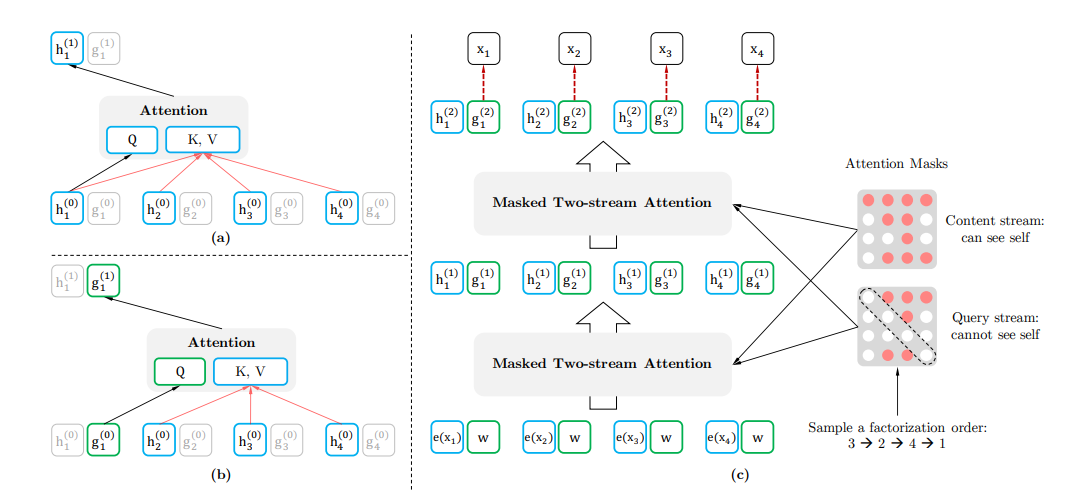
\includegraphics[width = 12cm]{figure/xlnet}\\ 
		{\tiny (a) content-stream; (b) query-stream; (c) whole model\\\footnotesize Source: \href{https://papers.nips.cc/paper/8812-xlnet-generalized-autoregressive-pretraining-for-language-understanding.pdf}{Yang et al. (2019)}}
	\end{figure}
\end{frame}



\begin{frame}{XLNet -- Model Input}

\textbf{Generation of samples:}

\begin{itemize}
\item Randomly sample two sentences and use concatenation* as input
			{\footnotesize
\begin{center}
\begin{tabular}{|cccccccc|}
\hline
\cellcolor{blue!15}\texttt{[CLS]} & The & fox & is & quick & . & \cellcolor{blue!15}\texttt{[SEP]} &\\\hline\hline It & jumps & over & the & lazy & dog & . & \cellcolor{blue!15}\texttt{[SEP]} \\
\hline
\end{tabular}\\\mbox{}
\end{center}}
{\scriptsize *Nevertheless: XLNet does \textit{not} use the NSP objective }
\end{itemize}

\textbf{Additional encodings:}

\begin{itemize}
\item \textit{Relative} segment encodings:
	\begin{itemize}
		\item BERT adds absolute segment embeddings ($E_A$ \& $E_B$)
		\item XLNet uses relative encodings ($\vec{s}_+$ \& $\vec{s}_-$)
	\end{itemize}
\item \textit{Relative} Positional encodings:
	\begin{itemize}
		\item BERT encodes information about the absolute position ($E_0, E_1, E_2, \hdots$)
		\item XLNet uses relative encodings ($R_{i - j}$)
	\end{itemize}
\end{itemize}
\end{frame}




\begin{frame}{XLNet -- Special remarks}
	
	\begin{itemize}
		\item \textbf{Partial Prediction:} Only predict the last tokens in a factoriztion order (reduces optimization difficulty)
					{\small $$\max_{\theta} \quad \mathds{E}_{\mathbf{z}\sim\mathcal{Z}_T} \left[ \sum_{t=c+1}^{|\mathbf{z}|} \log p_\theta (x_{z_t} | \mathbf{x}_{\mathbf{z}_{< t}}) \right],\quad \mbox{with $c$ as cutting point}$$}
		\item \textbf{Segment recurrence mechanism:} Allow for learning extended contexts in Transformer-based architectures, see \href{https://arxiv.org/pdf/1901.02860.pdf}{\beamergotobutton{Dai et al. (2019)}}
		\item \textbf{No independence assumption:}
	\begin{figure}
		\centering
		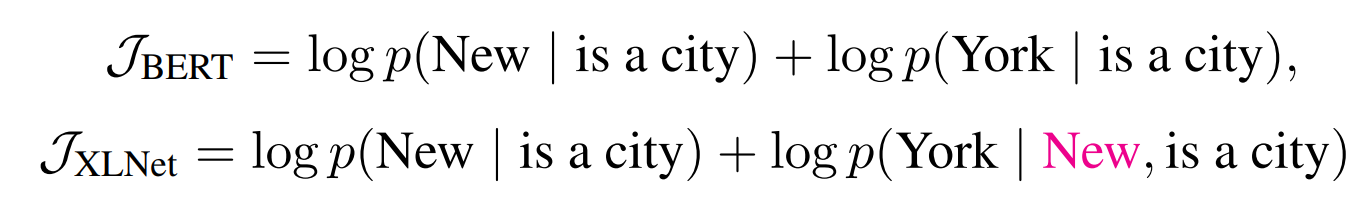
\includegraphics[width = 9cm]{figure/xlnet-objective}\\ 
		{\tiny Prediction of [New, York] given the factorization order [is, a, city, New, York]\\\footnotesize Source: \href{https://papers.nips.cc/paper/8812-xlnet-generalized-autoregressive-pretraining-for-language-understanding.pdf} \it Yang et al. (2019)}
	\end{figure}
	\end{itemize}
\end{frame}



\begin{frame}{XLNet -- SOTA performance}
\small
	\textbf{Performance differences to BERT:}

	\begin{figure}
		\centering
		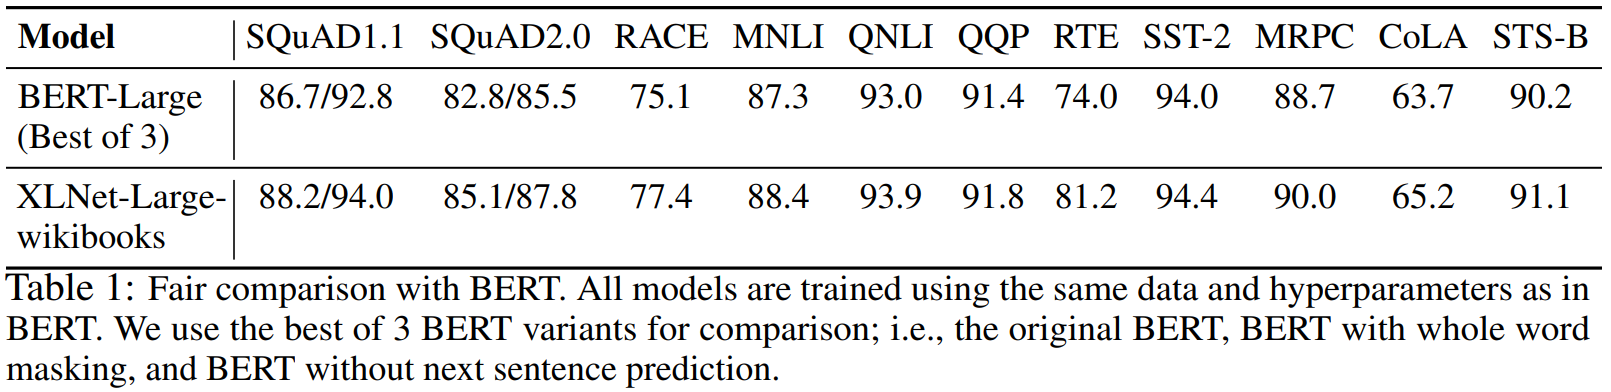
\includegraphics[width = 9cm]{figure/xlnet-vs-bert.png}\\ 
		\footnotesize{Source:} \href{https://papers.nips.cc/paper/8812-xlnet-generalized-autoregressive-pretraining-for-language-understanding.pdf}{\footnotesize Yang et al. (2019)}
	\end{figure}

	\textbf{SOTA performance:}

	\begin{figure}
		\centering
		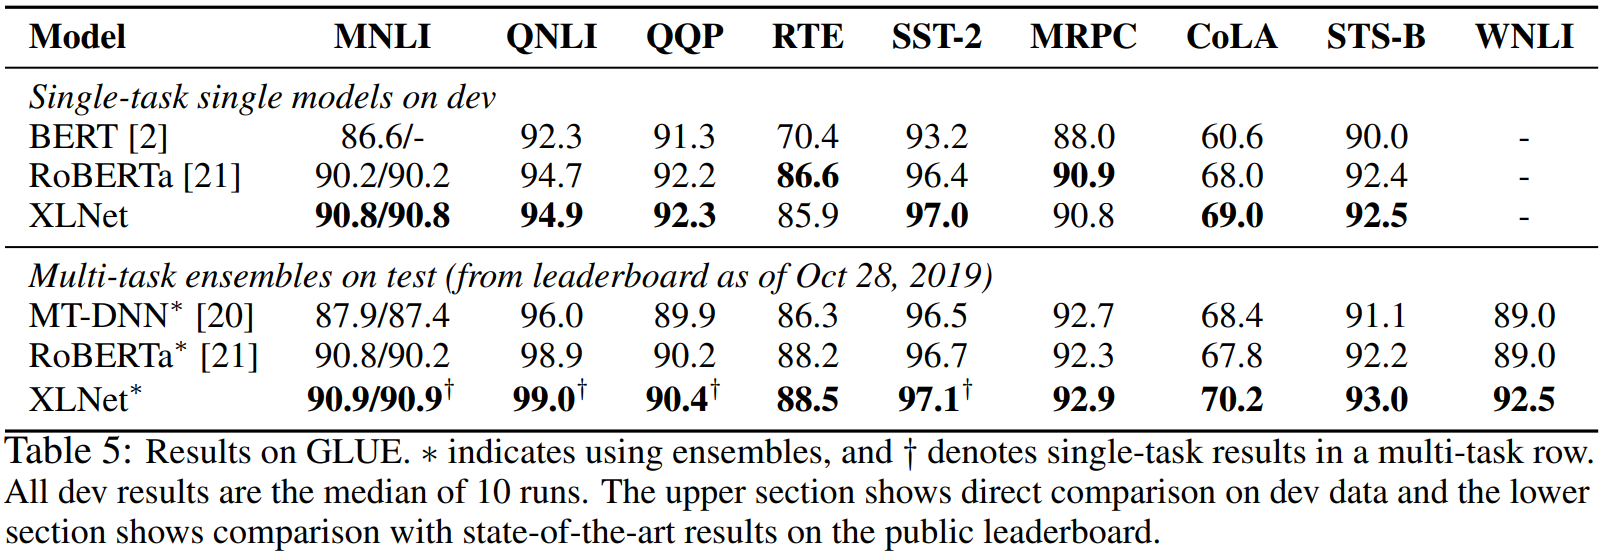
\includegraphics[width = 9cm]{figure/xlnet-sota.png}\\ 
		\footnotesize{Source:} \href{https://papers.nips.cc/paper/8812-xlnet-generalized-autoregressive-pretraining-for-language-understanding.pdf}{\footnotesize Yang et al. (2019)}
	\end{figure}
\end{frame}



\begin{frame}{Google's T5 \href{https://arxiv.org/pdf/1910.10683.pdf}{\beamergotobutton{Raffel et al. (2019)}}}

	\textbf{T5: Text-to-Text Transfer Transformer:}

	\begin{itemize}
		\item A complete encoder-decoder Transformer architecture
		\item All tasks reformulated as text-to-text tasks
		\item From BERT-size up to 11 Billion parameters
	\end{itemize}
	
	\begin{figure}
		\centering
		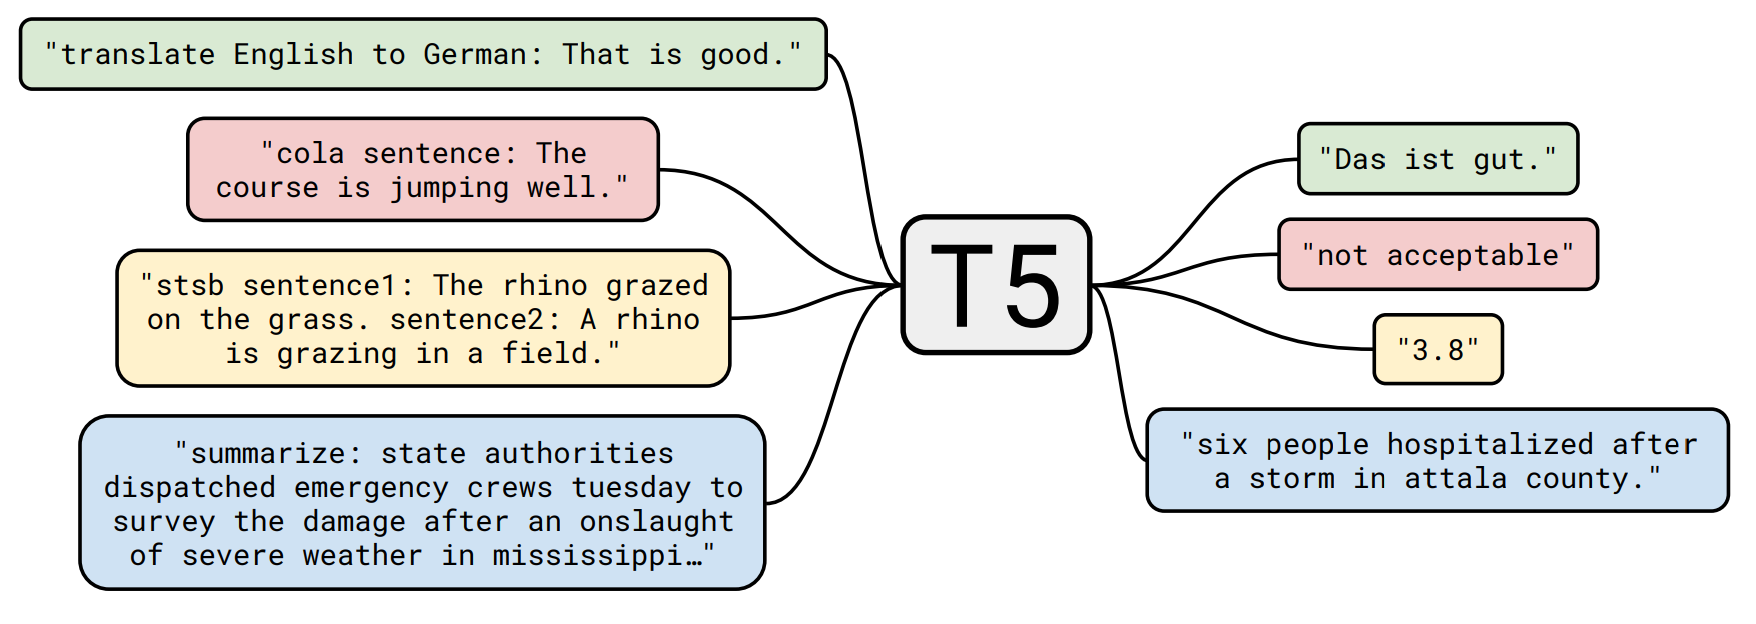
\includegraphics[width = 11cm]{figure/t5.png}\\ 
		\footnotesize{Source:} \href{https://arxiv.org/pdf/1910.10683.pdf}{\footnotesize Raffel et al. (2019)}
	\end{figure}
\end{frame}



\begin{frame}{T5 -- The \textbf{C}olossal \textbf{C}lean \textbf{C}rawled \textbf{C}orpus (C4)}
\small
	\begin{itemize}
		\item Effort to measure the effect of quality, characteristics \& size of the pre-training resources
		\item Common Crawl as basis, careful cleaning and filtering for English language
		\item Orders of magnitude larger (750GB) compared to commonly used corpora 
	\end{itemize}

	\vspace{.3cm}
	
	\textbf{Experiments (with respect to C4)}
	
	\begin{figure}
		\centering
		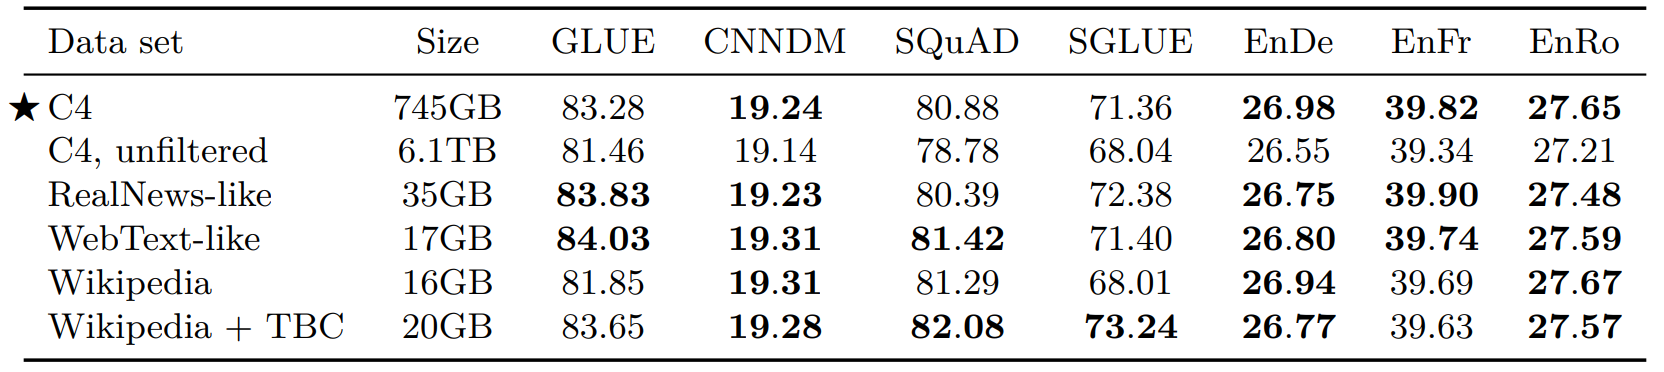
\includegraphics[width = 9cm]{figure/c4-characteristics.png}\\ 
		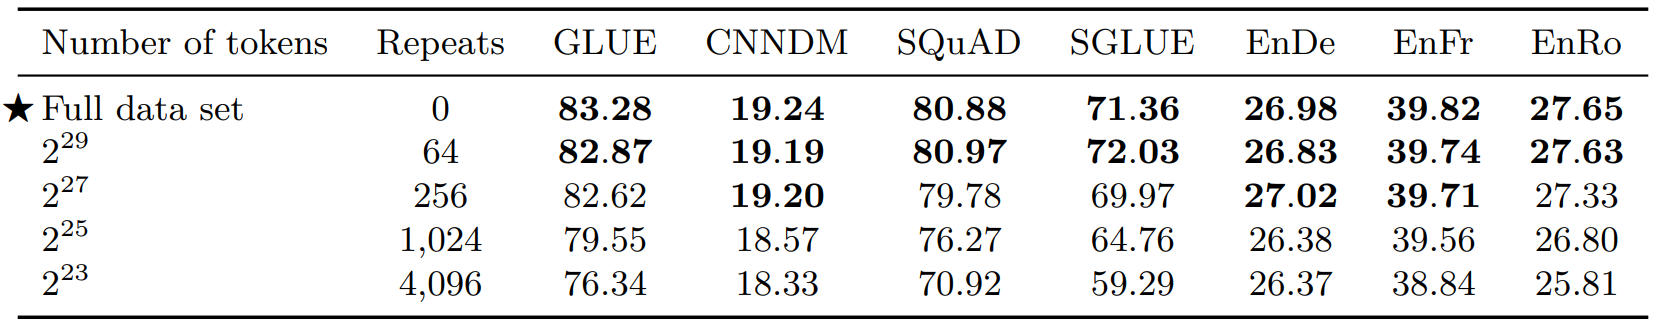
\includegraphics[width = 9cm]{figure/c4-size.png}\\ 
		\footnotesize{Source:} \href{https://arxiv.org/pdf/1910.10683.pdf}{\footnotesize Raffel et al. (2019)}
	\end{figure}
\end{frame}



\begin{frame}{T5 - Exhaustive Experiments}
\small
	\textbf{Performed experiments with respect to ..}
	
	\begin{itemize}
		\item .. architecture, size \& objective
		\item .. details of the Denoising objective
		\item .. fine-tuning methods \& multi-taks learning strategies
	\end{itemize}
	
	\textbf{Conclusions}
	
	\begin{itemize}
		\item Encoder-decoder architecture works best in this "text-to-text" setting
		\item More data, larger models \& ensembling all boost the performance
			\begin{itemize}
				\item Larger models trained for fewer steps better than smaller models on more data
				\item Ensembling: Using same base pre-trained models worse than complete separate model ensembles
			\end{itemize}
		\item Different denoising objectives work similarly well
		\item Updating \textit{all} model parameters during fine-tuning works best (but expensive)
	\end{itemize}
\end{frame}



\begin{frame}{ELECTRA \href{https://arxiv.org/pdf/2003.10555.pdf}{\beamergotobutton{Clark et al. (2020)}}}

	\textbf{ELECTRA: a different pre-training objective}

	\begin{itemize}
		\item (Small) generator model $G$ + (large) Discriminator model $D$
		\item Generator task: Masked language modeling
		\item Discriminator task: \textit{Replaced token detection}
		\item ELECTRA learns from \textit{all} of the tokens (not just from a small portion, like e.g. BERT)
	\end{itemize}
	
	\begin{figure}
		\centering
		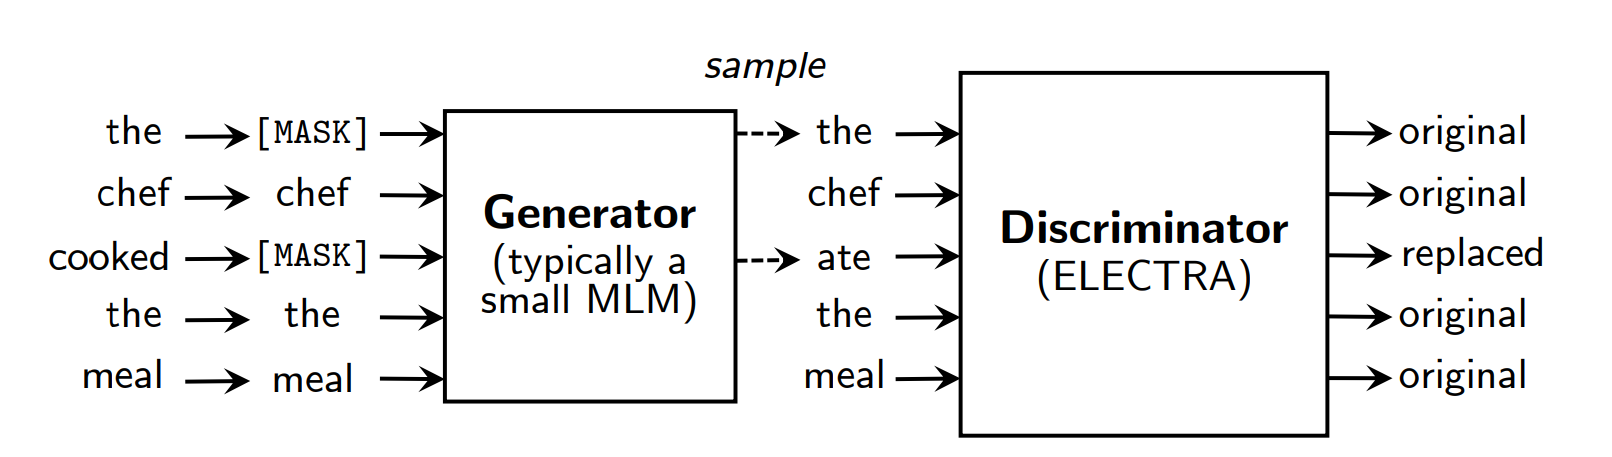
\includegraphics[width = 11cm]{figure/electra.png}\\ 
		\footnotesize{Source:} \href{https://arxiv.org/pdf/2003.10555.pdf}{\footnotesize Clark et al. (2020)}
	\end{figure}
\end{frame}



\begin{frame}{ELECTRA -- Training details}
	\textbf{Joint pre-training (but \textbf{not} in a GAN-fashion):}

	\begin{itemize}
		\item $G$ and $D$ are (Transformer) encoders which are trained jointly
		\item $G$ replaces \texttt{[MASK]}s in an input sequence\\
					$\rightarrow$ Passes corrupted input sequence $\vec{x}^{corrupt}$ to $D$
		\item \textit{Generation of samples:}
	\begin{figure}
		\centering
		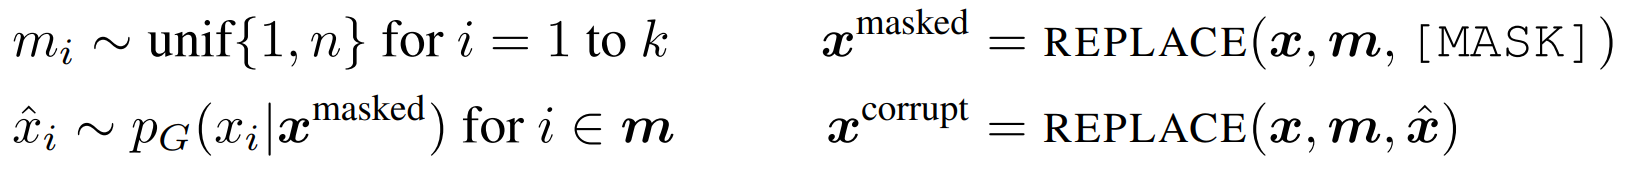
\includegraphics[width = 11cm]{figure/electra-samples.png}
	\end{figure}\vspace{-.25cm}
		{\footnotesize with approx. 15\% of the tokens masked out (via choice of $k$)}
		\item $D$ predicts whether $x_t,\; t \in 1, \hdots, T$ is "\textit{real}" or generated by $G$
			\begin{itemize}
				\item Softmax output layer for $G$ (probability distr. over all words)
				\item Sigmoid output layer for $D$ (Binary classification real vs. generated)
			\end{itemize}
	\end{itemize}
\end{frame}



\begin{frame}{ELECTRA -- Training details}

	Using the masked \& corrupted input sequences, the (joint) loss can be written down as follows:\\
	\vspace{.3cm}
	\textbf{Loss functions:}
	\begin{figure}
		\centering
		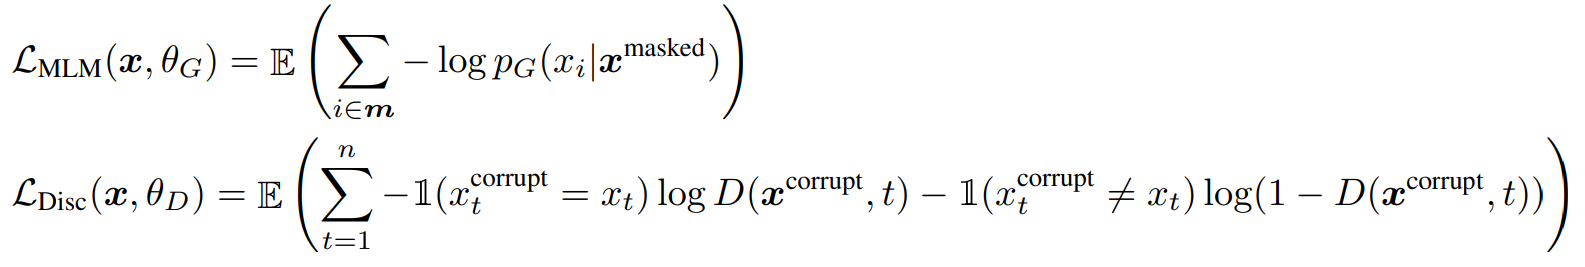
\includegraphics[width = 11cm]{figure/electra-loss.png}
	\end{figure}
	
	\textbf{Combined:}
	\begin{figure}
		\centering
		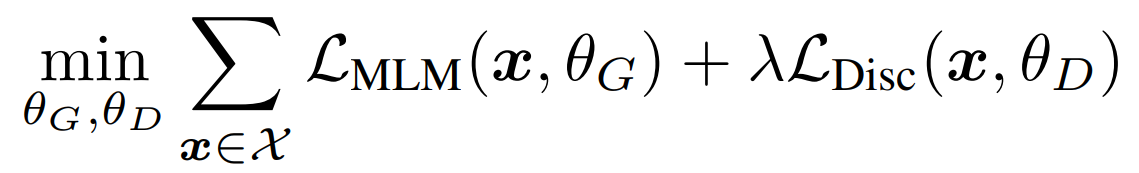
\includegraphics[width = 6cm]{figure/electra-loss-comb.png}
	\end{figure}
	{\footnotesize with $\lambda$ set to 50, since the discriminator's loss is typically much lower than the geneator's.}
\end{frame}



\begin{frame}{ELECTRA -- Training details}
\small
	\textbf{Generator size:}

	\begin{itemize}
		\item Same size of $G$ and $D$: 
			\begin{itemize}
				\item Twice as much compute per training step + too challenging for $D$
			\end{itemize}
		\item Smaller Generators are preferable (1/4 -- 1/2 the size of $D$)
	\begin{figure}
		\centering
		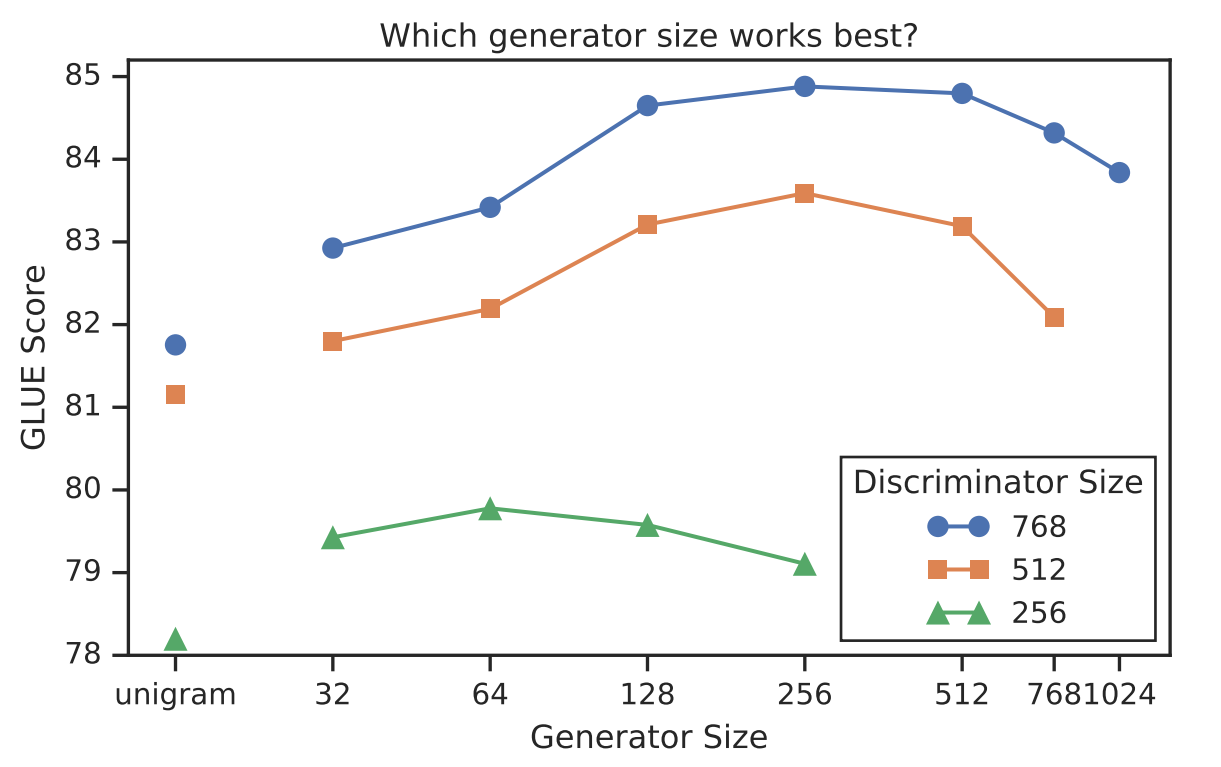
\includegraphics[width = 5cm]{figure/electra-size-g.png}\\ 
		\scriptsize{Source:} \href{https://arxiv.org/pdf/2003.10555.pdf}{\scriptsize Clark et al. (2020)}
	\end{figure}
	\end{itemize}
	
	\textbf{Weight sharing (experimental):}

	\begin{itemize}
		\item Same size of $G$ and $D$: All weights can be tied
		\item $G$ smaller than $D$: Share token \& positional embeddings 
	\end{itemize}
\end{frame}



\begin{frame}{ELECTRA -- Model comparison}
	
	\begin{figure}
		\centering
		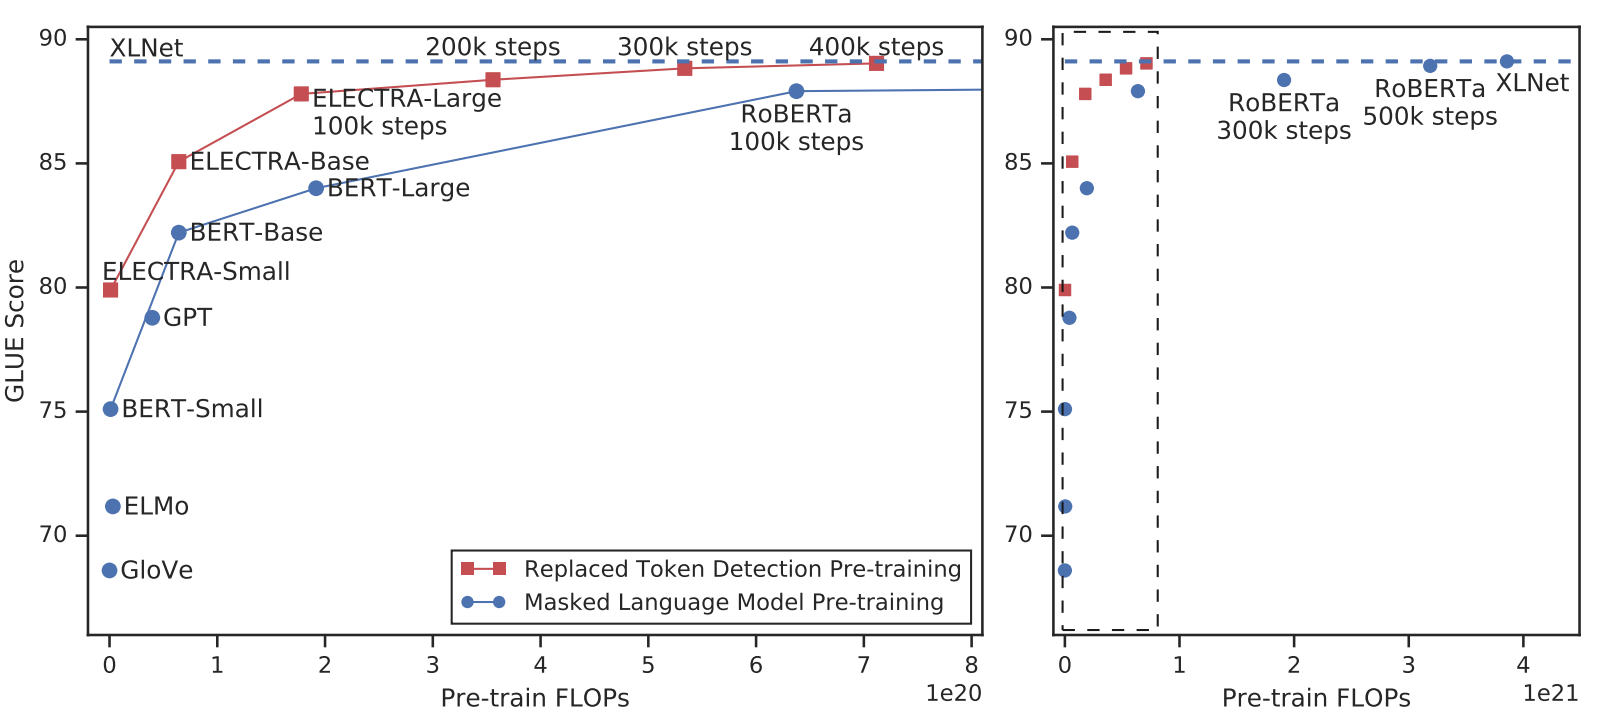
\includegraphics[width = 12cm]{figure/electra-glue.png}\\ 
		\footnotesize{Source:} \href{https://arxiv.org/pdf/2003.10555.pdf}{\footnotesize Clark et al. (2020)}
	\end{figure}
	
{\footnotesize \textit{Note:} Different batch sizes (2k vs. 8k) for ELECTRA vs. RoBERTa/XLNet explain why same number of steps lead to approx. 1/4 of the compute for ELECTRA.}
\end{frame}



\begin{frame}{ELECTRA -- SOTA performance}
\small
	\textbf{Performance differences vs. BERT/RoBERTa (GLUE dev set):}

	\begin{figure}
		\centering
		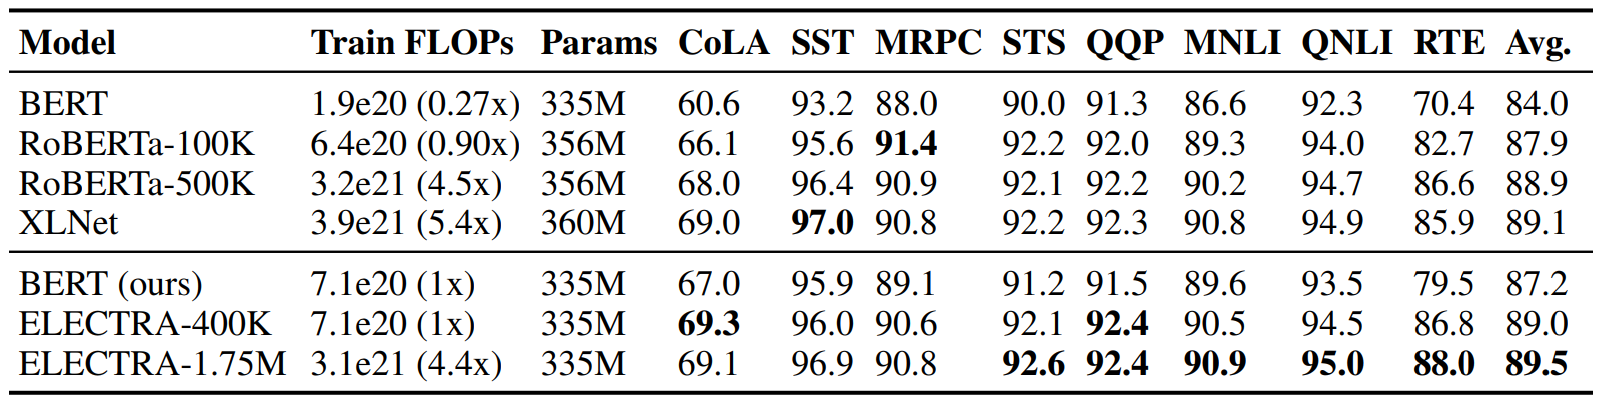
\includegraphics[width = 9cm]{figure/electra-sota1.png}\\ 
		{\footnotesize Source: \href{https://arxiv.org/pdf/2003.10555.pdf}{Clark et al. (2020)}}
	\end{figure}

	\textbf{SOTA performance (GLUE test set):}

	\begin{figure}
		\centering
		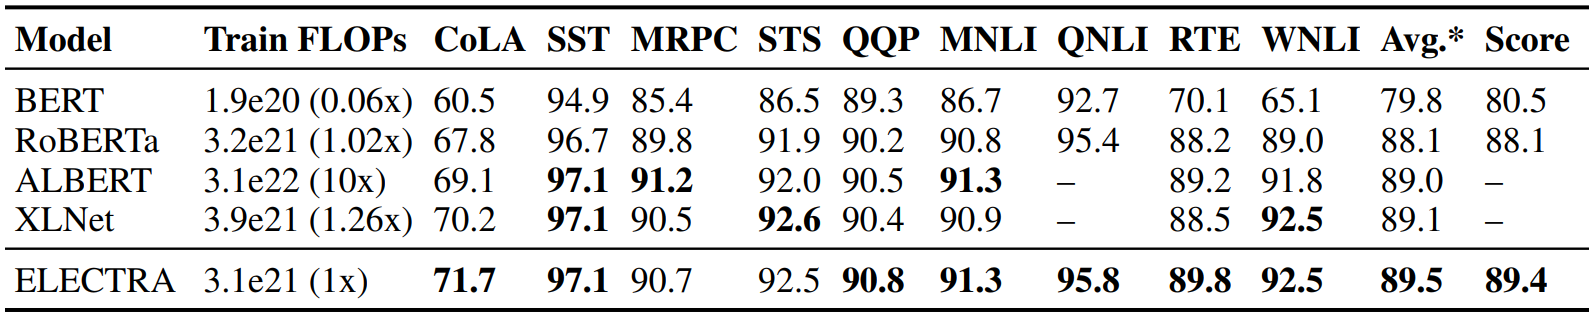
\includegraphics[width = 9cm]{figure/electra-sota2.png}\\ 
		{\tiny * Avg. excluding QNLI to ensure comparability\\\footnotesize Source: \href{https://arxiv.org/pdf/2003.10555.pdf}{Clark et al. (2020)}}
	\end{figure}
\end{frame}



\begin{frame}{Model distillation \href{https://arxiv.org/pdf/1503.02531.pdf}{\beamergotobutton{Hinton et al. (2015)}}}

\textbf{Model compression scheme:}

\begin{itemize}
	\item Motivation comes from having computationally expensive, cumbersome ensemble models. \href{http://www.niculescu-mizil.org/papers/rtpp364-bucila.rev2.pdf}{\beamergotobutton{Bucila et al. (2006)}}
	\item Compressing the knowlegde of the ensemble into a single model has the benefit of easier deployment and better generalization
	\item Reasoning:
		\begin{itemize}
			\item Cumbersome model generalizes well, because it is the average of an ensemble.
			\item Small model trained to generalize in the same way typically better than small model trained "the normal way".
		\end{itemize}
\end{itemize}

\textbf{Distillation:}

\begin{itemize}
	\item Temperature $T$ in the softmax: $q_i = \frac{\exp(z_i/T)}{\sum_j \exp(z_j/T)}$
	\item Knowledge transfer via soft targets with high $T$ from original model.
	\item When true labels are known: Weighted average of two different objective functions
\end{itemize}

	
\end{frame}



\begin{frame}{DistilBERT \href{https://arxiv.org/pdf/1910.01108.pdf}{\beamergotobutton{Sanh et al. (2019)}}}

\textbf{Motivation:}
	\begin{figure}
		\centering
		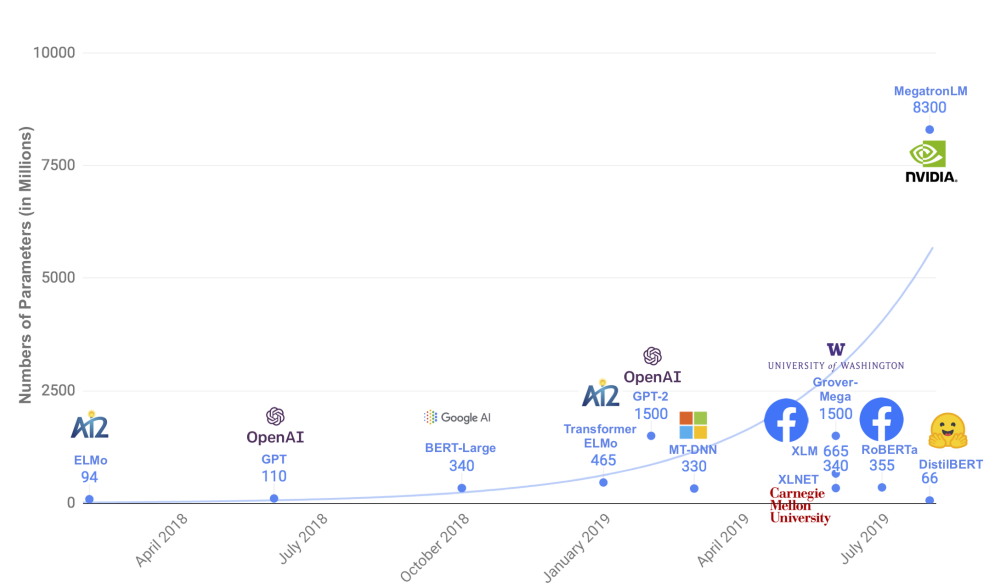
\includegraphics[width = 11cm]{figure/distilbert-motivation}\\ 
		{\footnotesize Source: \href{https://arxiv.org/pdf/1910.01108.pdf}{Sanh et al. (2019)}}
	\end{figure}
	
\end{frame}



\begin{frame}{DistilBERT \href{https://arxiv.org/pdf/1910.01108.pdf}{\beamergotobutton{Sanh et al. (2019)}}}

\textbf{Student architecture (\textit{DistilBERT}):}

\begin{itemize}
	\item Half the number of layers compared to BERT*
 	\item Half of the size of BERT, but retains 95\% of the performance
	\item Initialize from BERT (taking one out of two hidden layers)
	\item Same pre-training data as BERT (Wiki + BooksCorpus)
\end{itemize}

\vspace{.3cm}

\textbf{Training and performance}

\begin{itemize}
	\item Distillation loss $L_{ce} = \sum_i t_i \cdot \log(s_i)$ + MLM-Loss $L_{mlm}$ + \\
				Cosine-Embedding-Loss $L_{cos}$
	\item Drops NSP, use dynamic masking, train with large batches
\end{itemize}

\vspace{1cm}

{\footnotesize *Rationale for "only" reducing the number of layers:\\
Larger influence on the computation efficiency compared to e.g. hidden size dimension}
	
\end{frame}



\begin{frame}{DistilBERT \href{https://arxiv.org/pdf/1910.01108.pdf}{\beamergotobutton{Sanh et al. (2019)}}}
\small
	\textbf{Performance differences to BERT:}

	\begin{figure}
		\centering
		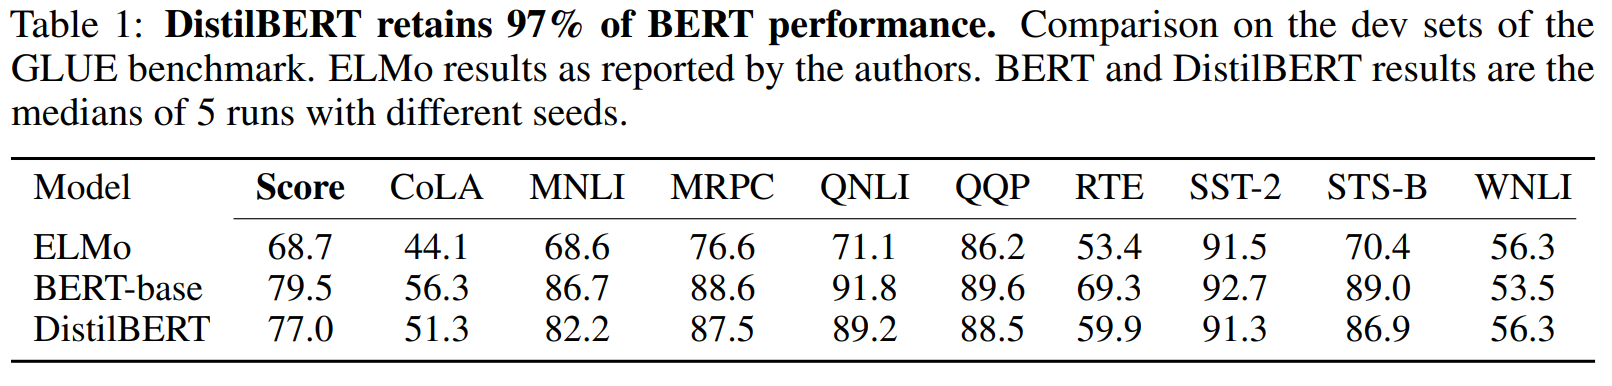
\includegraphics[width = 9cm]{figure/distilbert-vs-sota.png}\\ 
		\footnotesize{Source:} \href{https://arxiv.org/pdf/1910.01108.pdf}{\footnotesize Sanh et al. (2019)}
	\end{figure}

	\textbf{Ablation study regarding the loss:}

	\begin{figure}
		\centering
		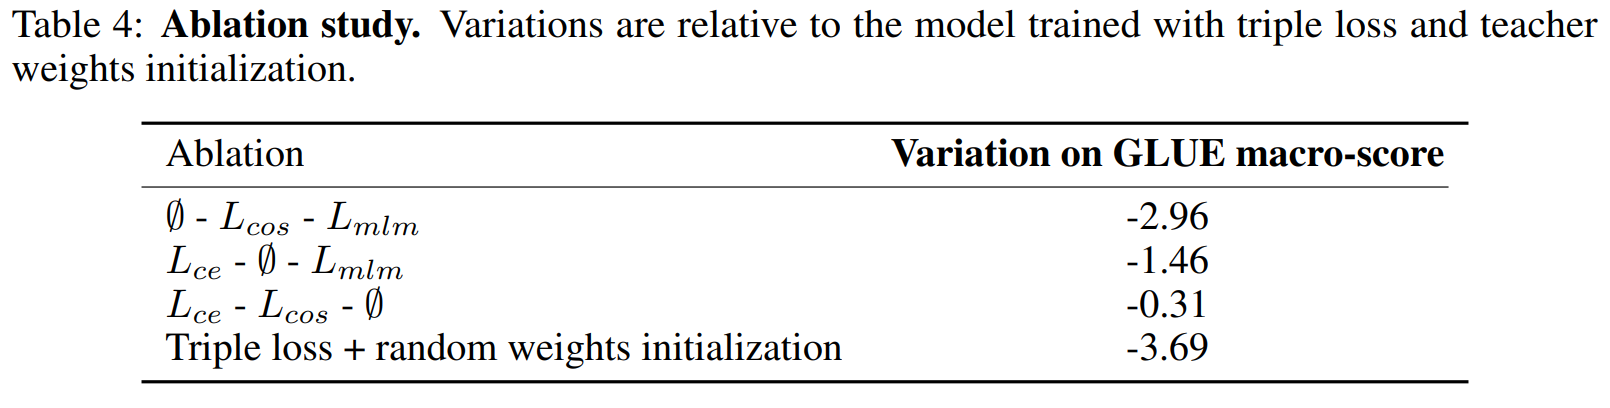
\includegraphics[width = 9cm]{figure/distilbert-ablation.png}\\ 
		\footnotesize{Source:} \href{https://arxiv.org/pdf/1910.01108.pdf}{\footnotesize Sanh et al. (2019)}
	\end{figure}
	
\end{frame}



\begin{frame}{The $\mathcal{O}(n^2)$ problem}

\textbf{Quadratic time \& memory complexity of Self-Attention}

\begin{itemize}
	\item \textit{Inductive bias of Transformer models:}\\
				Connect all tokens in a sequence to each other
	\item \textbf{Pro:} Can (theoretically) learn contexts of arbitrary length
	\item \textbf{Con:} Bad scalability limiting (feasible) context size
\end{itemize}

\vspace{.3cm}

\textbf{Resulting Problems:}

\begin{itemize}
	\item Several tasks require models to consume longer sequences
	\item \textit{Efficiency:} Are there more efficient modifications which achieve similar or even better performance? 
\end{itemize}
	
\end{frame}



\begin{frame}{Efficient Transformers \href{https://arxiv.org/pdf/2009.06732.pdf}{\beamergotobutton{Tay et al. (2020)}}}

\textbf{Broad overview on so-called "X-formers":}

\begin{itemize}
	\item Efficient \& fast Transformer-based models\\
				$\rightarrow$ Reduce complexity from $\mathcal{O}(n^2)$ to (up to) $\mathcal{O}(n)$
	\item Claim on-par (or even) superior performance
	\item Different techniques used:
				\begin{itemize}
					\item Fixed/Factorized/Random Patterns
					\item Learnable Patterns (extension of the above)
					\item Low-Rank approximations or Kernels
					\item Recurrence (see e.g. \href{https://arxiv.org/pdf/1901.02860.pdf}{\beamergotobutton{Transformer-XL (Dai et al., 2019)}})
					\item Memory modules
				\end{itemize}
\end{itemize}
	
	\vspace{.3cm}
	
\textbf{Side note:}

\begin{itemize}
	\item Most Benchmark data sets not explicitly designed for evaluating long-range abilities of the models.
	\item Recently proposed: \href{https://arxiv.org/pdf/2011.04006.pdf}{\beamergotobutton{\textit{Longe Range Arena: A benchmark for efficient transformers} (Tay et al., 2020)}}
\end{itemize}
	
\end{frame}



\begin{frame}{Introducing Patterns}

\textbf{Reasoning:} 

\begin{itemize}
	\item Making every token attend to every other token might be unnecessary
	\item Introduce sparsity in the commonly dense attention matrix
\end{itemize}

\textbf{Example:}

	\begin{figure}
		\centering
		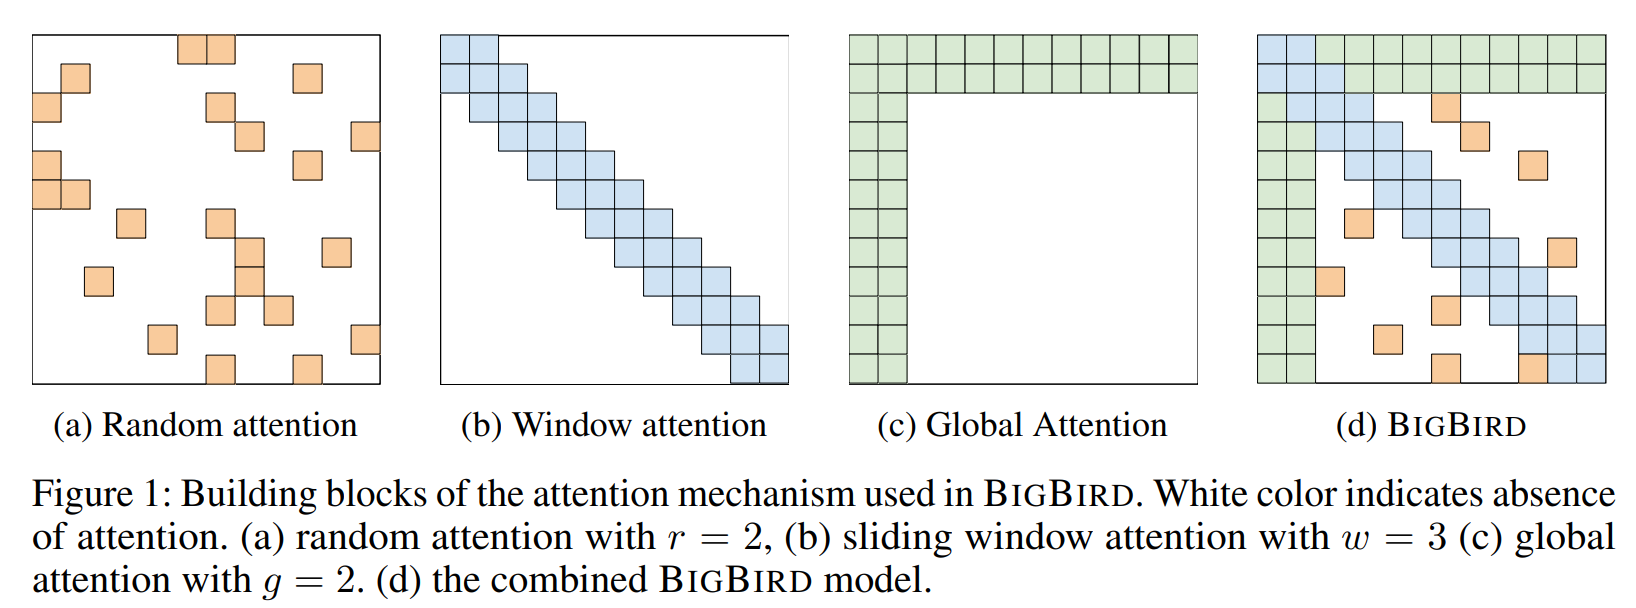
\includegraphics[width = 11cm]{figure/bigbird-patterns.png}\\ 
		{\footnotesize Source: \href{https://proceedings.neurips.cc//paper/2020/file/c8512d142a2d849725f31a9a7a361ab9-Paper.pdf}{Zaheer et al. (2020)}}
	\end{figure}
\end{frame}



\begin{frame}{Linear Self-Attention \href{https://arxiv.org/pdf/2006.04768.pdf}{\beamergotobutton{Wang et al. (2020)}}}

\textbf{Reasoning:} 

\begin{itemize}
	\item Most information in the Self-Attention mechanism can be recovered from the first few, largest singular values
	\item Introduce additional $k$-dimensional projection before self-attention
\end{itemize}

	\begin{figure}
		\centering
		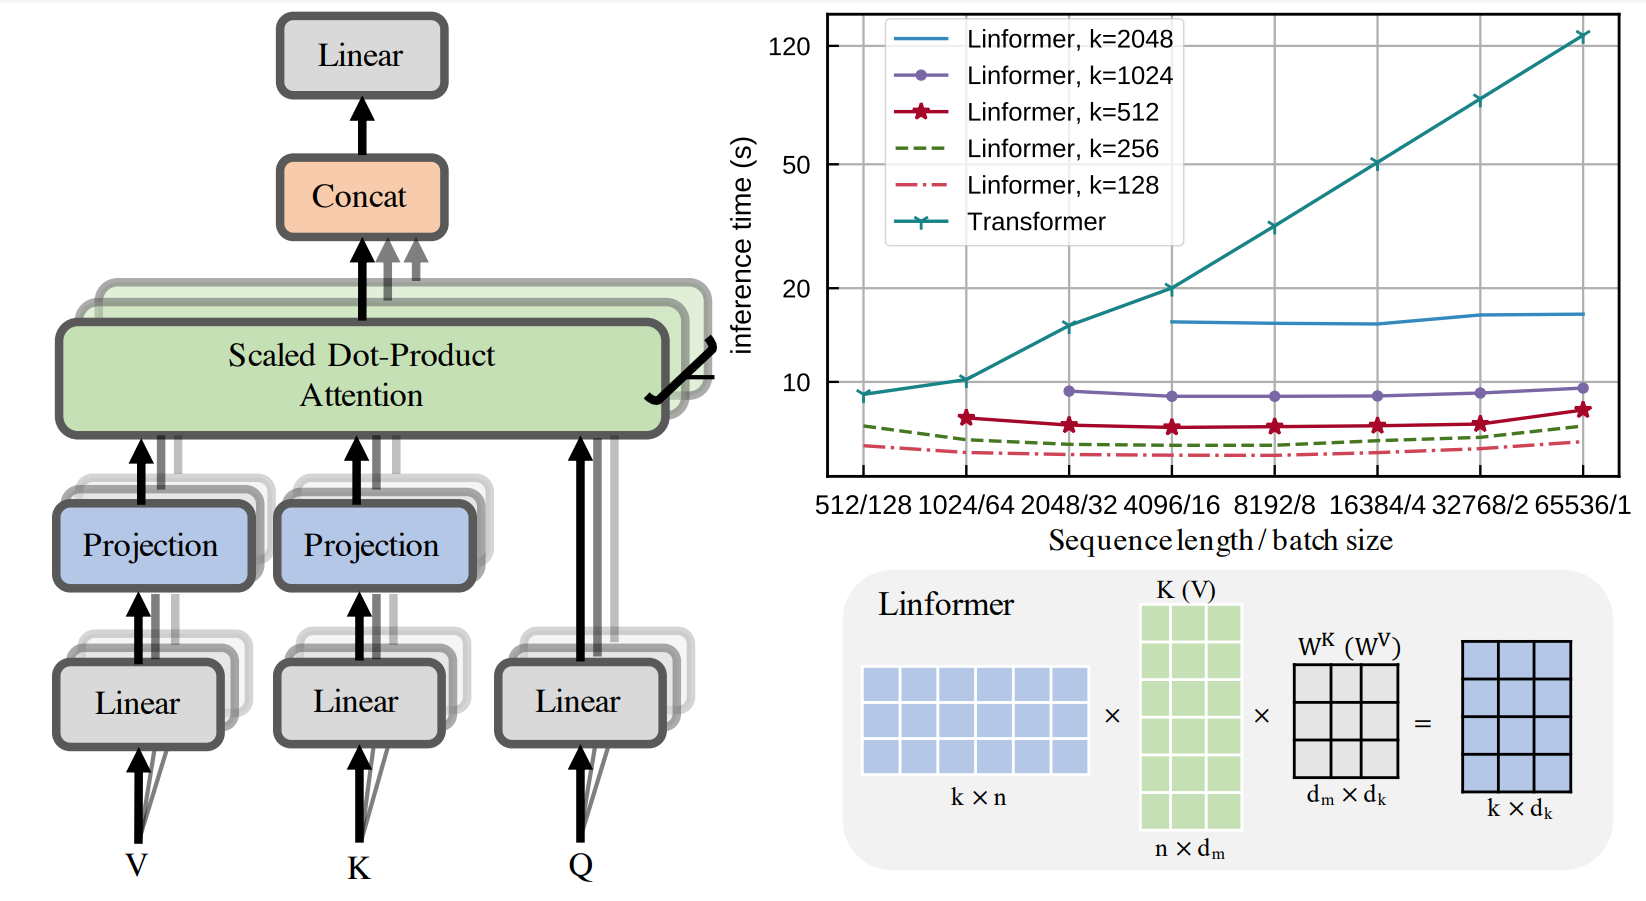
\includegraphics[width = 8cm]{figure/linformer.png}\\ 
		{\footnotesize Source: \href{https://arxiv.org/pdf/2006.04768.pdf}{Wang et al. (2020)}}
	\end{figure}
\end{frame}



\begin{frame}{DeBERTa \href{https://arxiv.org/pdf/2006.03654.pdf}{\beamergotobutton{He et al. (2020)}}}
\small
	\textbf{Disentangled Attention:}
	\begin{itemize}
		\item Each token represented by two vectors for content ($\mathbf{H}_i$) and relative position ($\mathbf{P}_{i|j}$) 
		\item Calculation of the Attention Score:
	\begin{figure}
		\centering
		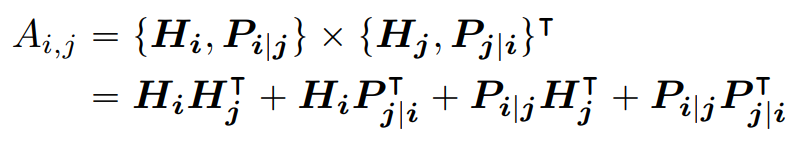
\includegraphics[width = 7cm]{figure/deberta-attn.png}
	\end{figure}
		\item with content-to-content, content-to-position, position-to-content and position-to-position attention
	\end{itemize}
\end{frame}



\begin{frame}{Disentangled Attention}
	\textbf{Standard (Single-head) Self-Attention:}

	\begin{figure}
		\centering
		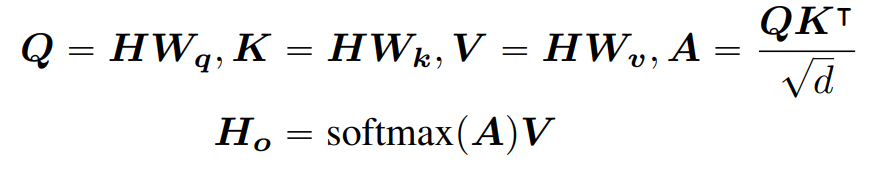
\includegraphics[width = 7cm]{figure/deberta-single.png}
	\end{figure}
	
	\textbf{Disentangled Attention*:}

	\begin{figure}
		\centering
		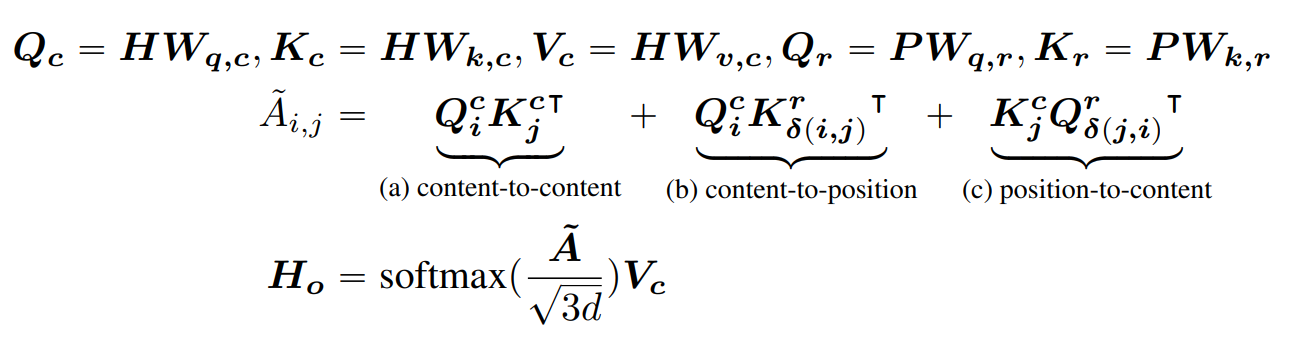
\includegraphics[width = 10cm]{figure/deberta-dis.png}
	\end{figure}
	

{\footnotesize *Position-to-position part is removed since it, according to the authors, does not provide much additional information as \textit{relative} position emebeddings are used.}
\end{frame}



\begin{frame}{Further reading}

	\begin{itemize}
		\item BART \href{https://arxiv.org/pdf/1910.13461.pdf}{\beamergotobutton{Lewis et al. (2019)}}
		\item BORT \href{https://arxiv.org/pdf/2010.10499.pdf}{\beamergotobutton{de Wynter \& Perry (2020)}}
		\item WT5?! \href{https://arxiv.org/pdf/2004.14546.pdf}{\beamergotobutton{Narang et al. (2020)}}
	\end{itemize}
	
\end{frame}


\end{document}



\begin{frame}{}
	
\end{frame}